\documentclass[aspectratio=169]{beamer}

\pdfminorversion=7

\usepackage[english]{babel}
\usepackage[T1]{fontenc} % For æ, ø and å
\usepackage[utf8]{inputenc}

\usepackage{ae,aecompl}
\usepackage{pslatex}

\usepackage[export]{adjustbox}

\setbeamertemplate{navigation symbols}{}

\begin{document}

%%% Hyperfocal distance

\begin{frame}[plain]{}
  \vspace{3ex}
  \begin{center} \LARGE \bf
    Hyperfocal distance
  \end{center}
\end{frame}

\begin{frame}[plain]{}
  \vspace{1ex}
  \centering
  Hyperfocal distance | Sony $\alpha$\hspace{0.1em}6000 (aps-c) | CoC = 0.036 mm
  
  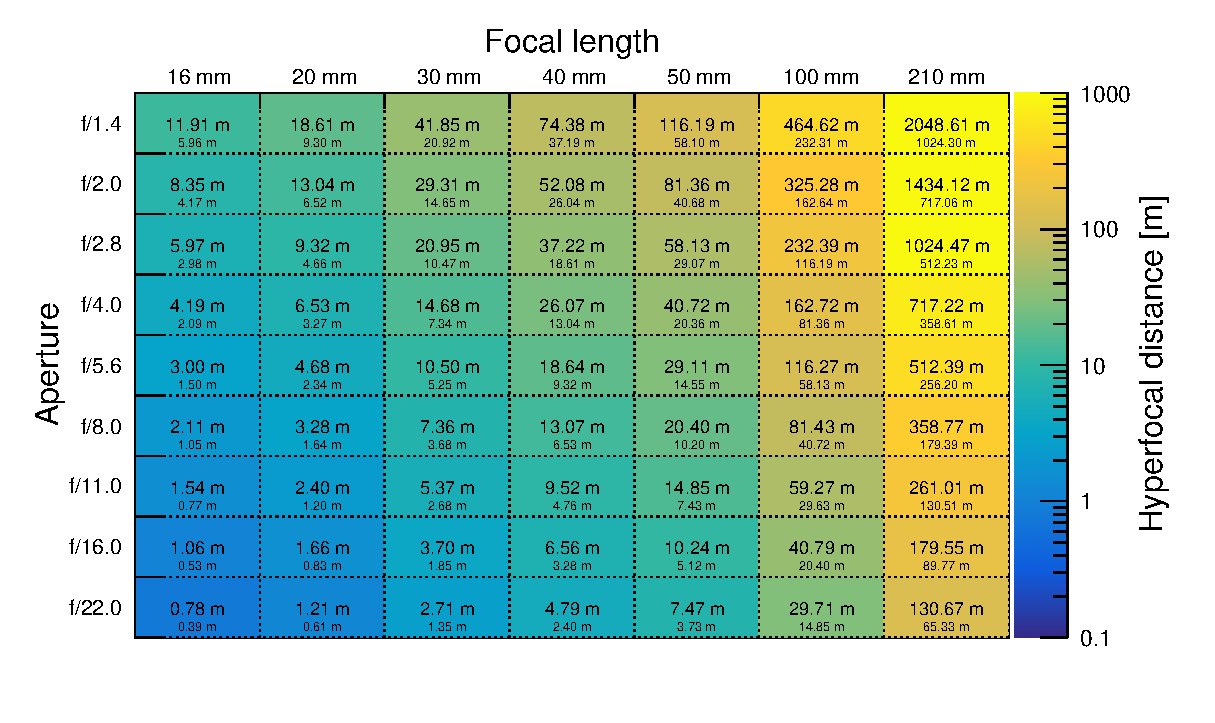
\includegraphics[center,width=0.78\textwidth]{img/hyperfocal-distance.eps}
\end{frame}

%%% Depth of Field

\begin{frame}[plain]{}
  \vspace{3ex}
  \begin{center} \LARGE \bf
    Depth of Field
  \end{center}
\end{frame}

\begin{frame}[plain]{}
  \vspace{1ex}
  \centering
  Depth of Field | {\bf Focal length = 16 mm} |  Sony $\alpha$\hspace{0.1em}6000 (aps-c) | CoC = 0.036 mm
  
  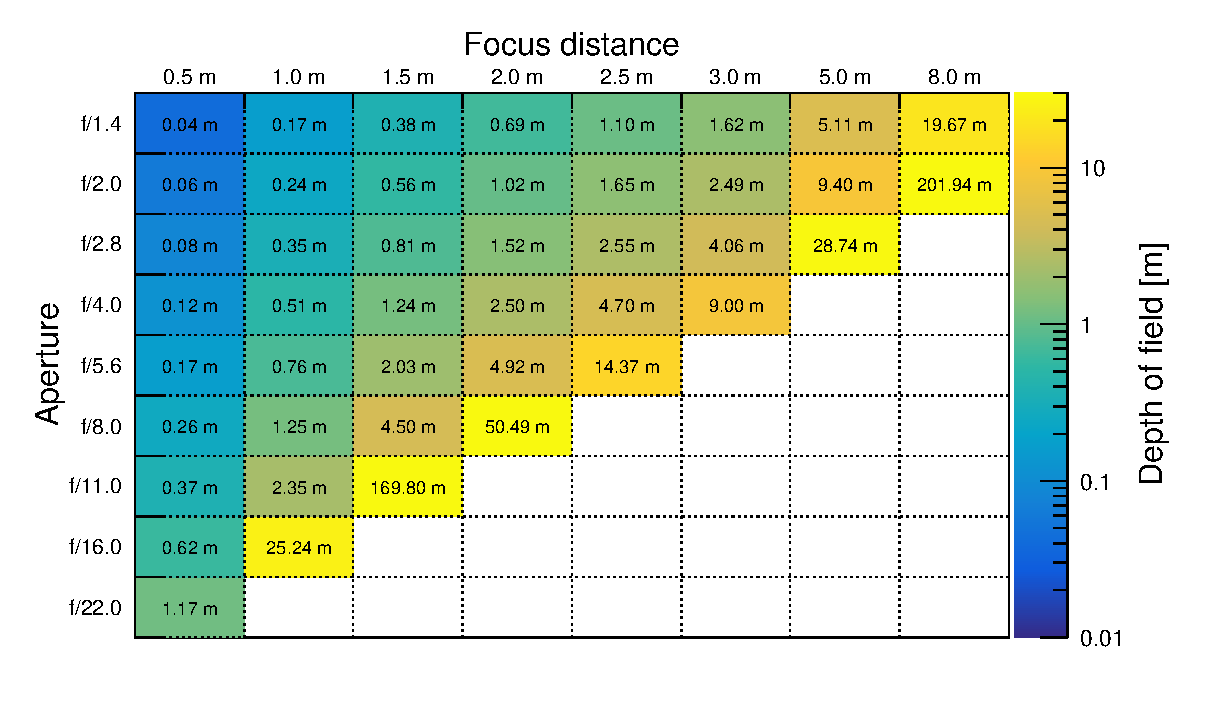
\includegraphics[center,width=0.78\textwidth]{img/depth-of-field_focl16.eps}
\end{frame}

\begin{frame}[plain]{}
  \vspace{1ex}
  \centering
  Depth of Field | {\bf Focal length = 20 mm} |  Sony $\alpha$\hspace{0.1em}6000 (aps-c) | CoC = 0.036 mm
  
  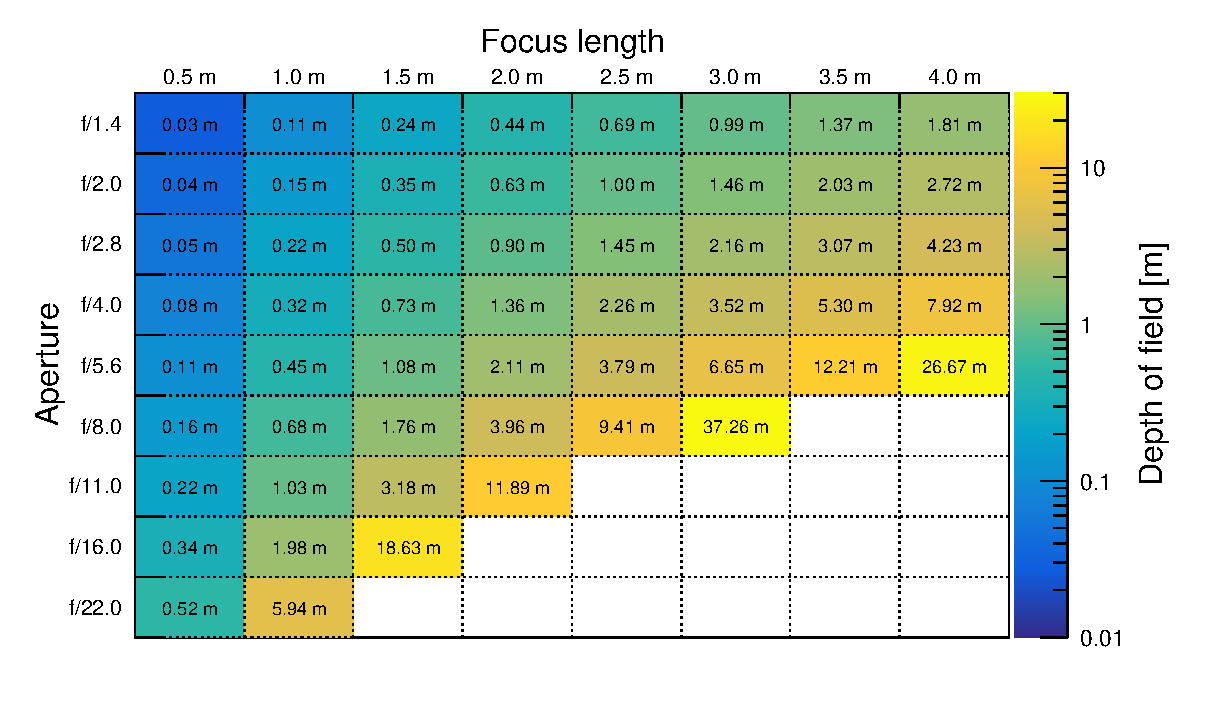
\includegraphics[center,width=0.78\textwidth]{img/depth-of-field_focl20.eps}
\end{frame}

\begin{frame}[plain]{}
  \vspace{1ex}
  \centering
  Depth of Field | {\bf Focal length = 30 mm} |  Sony $\alpha$\hspace{0.1em}6000 (aps-c) | CoC = 0.036 mm
  
  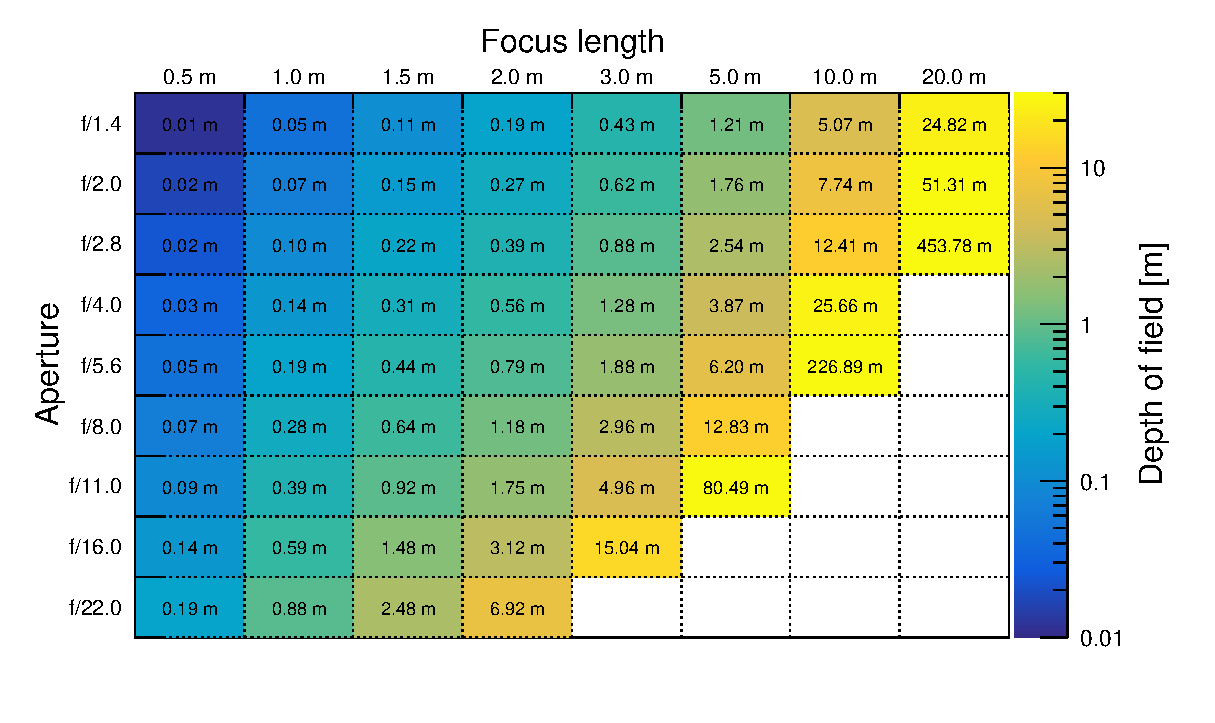
\includegraphics[center,width=0.78\textwidth]{img/depth-of-field_focl30.eps}
\end{frame}

\begin{frame}[plain]{}
  \vspace{1ex}
  \centering
  Depth of Field | {\bf Focal length = 40 mm} |  Sony $\alpha$\hspace{0.1em}6000 (aps-c) | CoC = 0.036 mm
  
  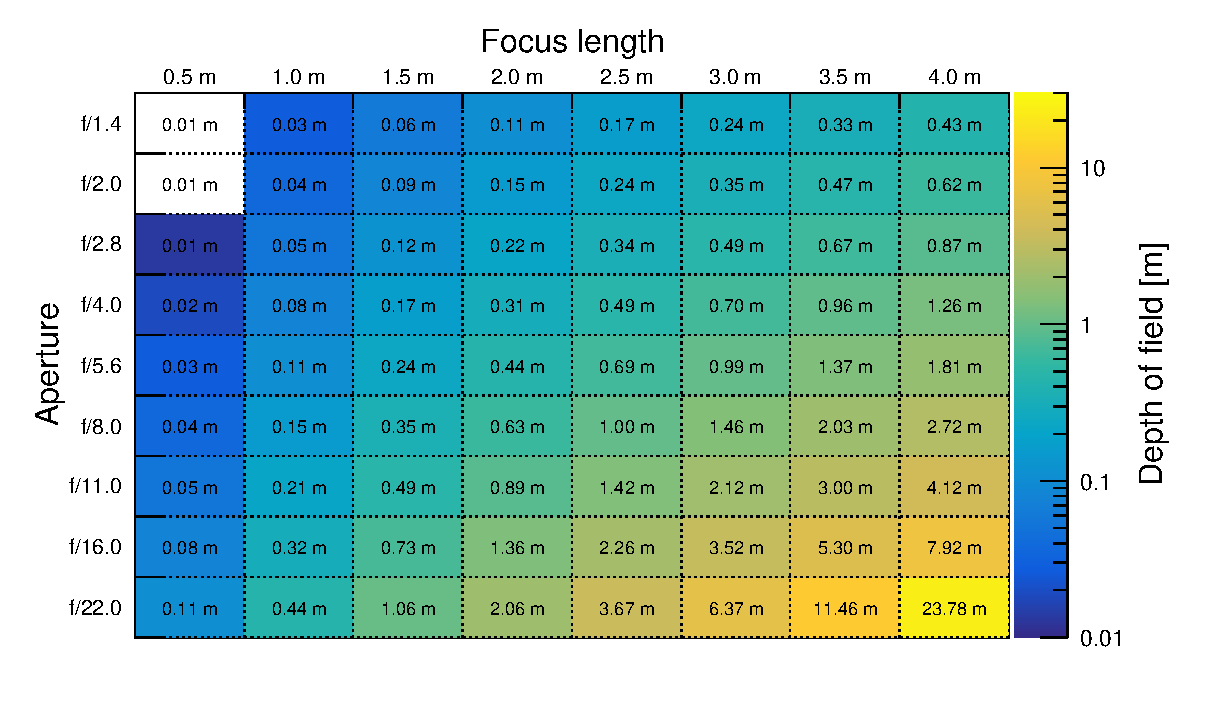
\includegraphics[center,width=0.78\textwidth]{img/depth-of-field_focl40.eps}
\end{frame}

\begin{frame}[plain]{}
  \vspace{1ex}
  \centering
  Depth of Field | {\bf Focal length = 50 mm} |  Sony $\alpha$\hspace{0.1em}6000 (aps-c) | CoC = 0.036 mm
  
  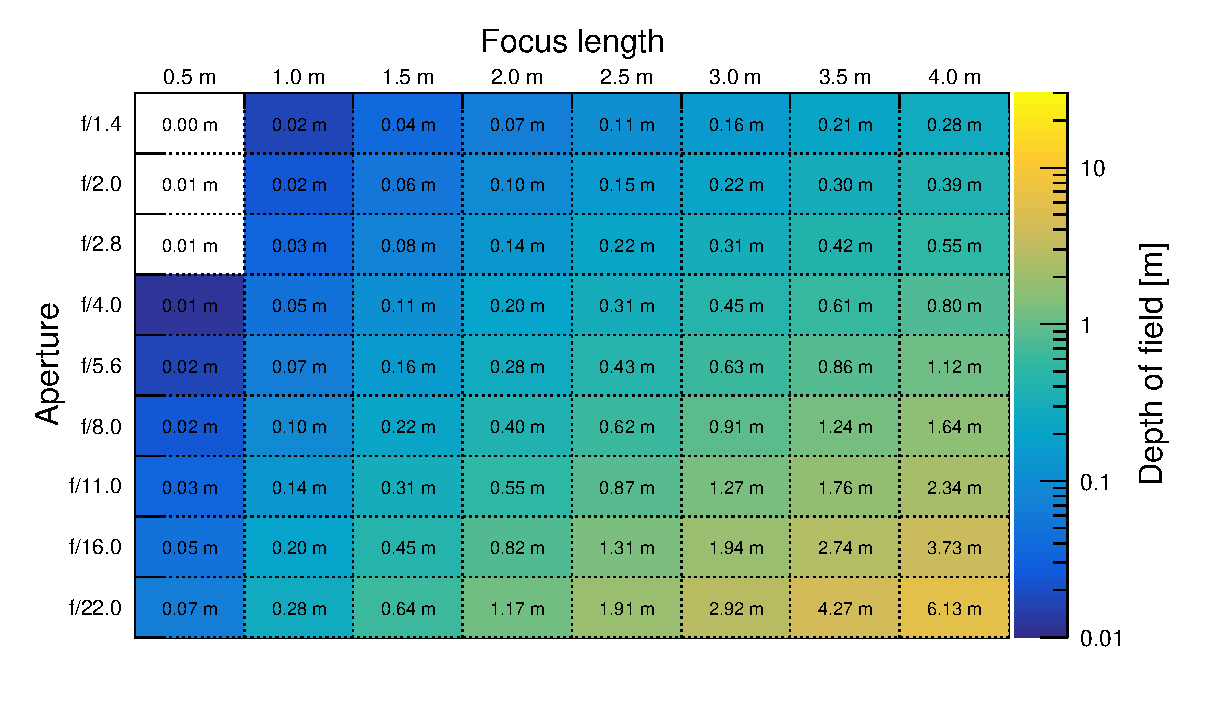
\includegraphics[center,width=0.78\textwidth]{img/depth-of-field_focl50.eps}
\end{frame}

\begin{frame}[plain]{}
  \vspace{1ex}
  \centering
  Depth of Field | {\bf Focal length = 100 mm} |  Sony $\alpha$\hspace{0.1em}6000 (aps-c) | CoC = 0.036 mm
  
  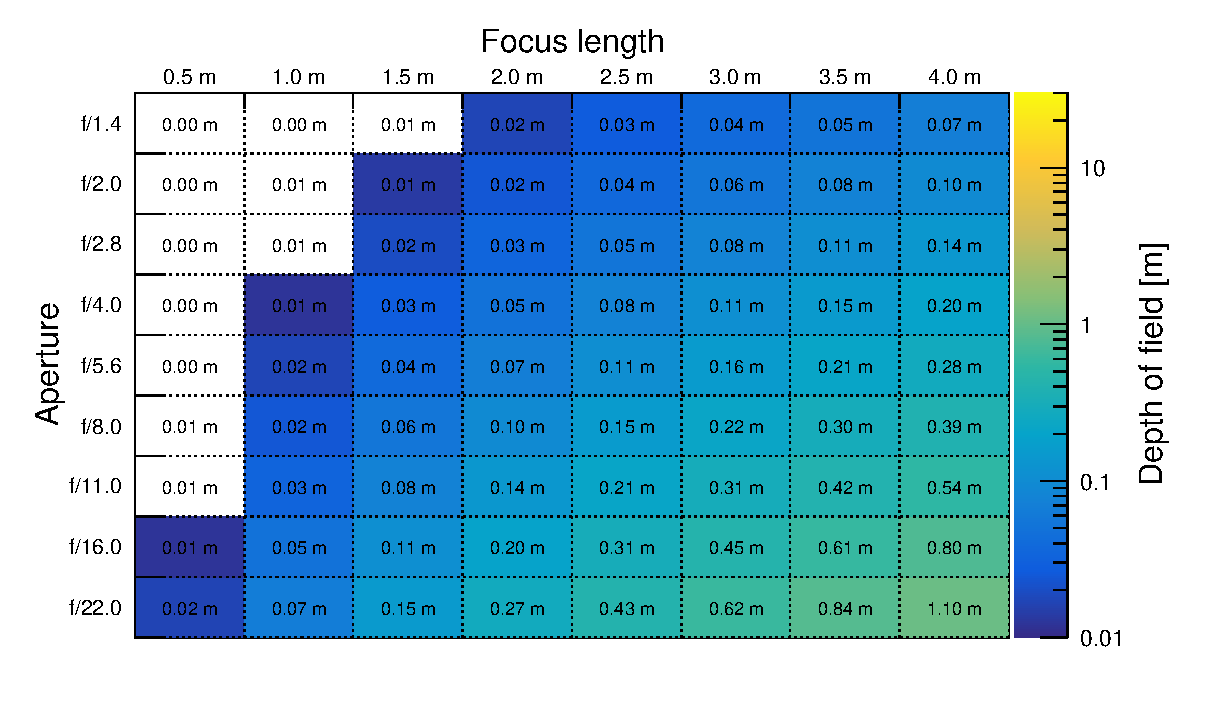
\includegraphics[center,width=0.78\textwidth]{img/depth-of-field_focl100.eps}
\end{frame}

\begin{frame}[plain]{}
  \vspace{1ex}
  \centering
  Depth of Field | {\bf Focal length = 210 mm} |  Sony $\alpha$\hspace{0.1em}6000 (aps-c) | CoC = 0.036 mm
  
  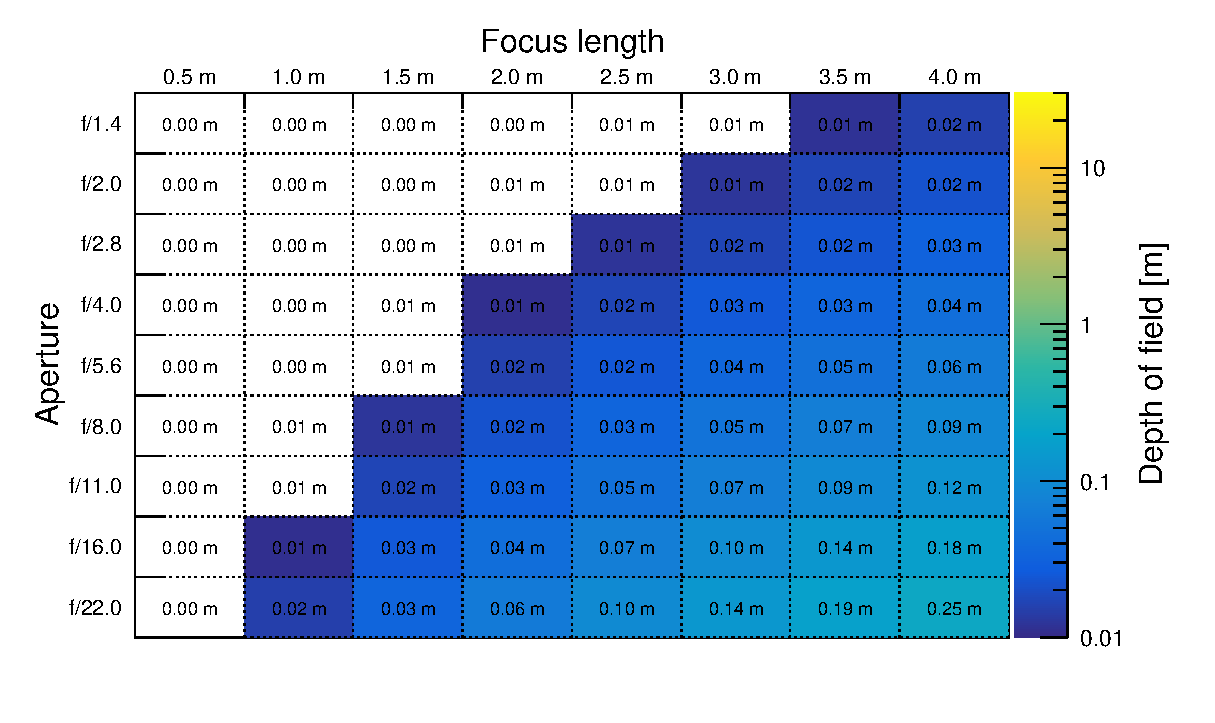
\includegraphics[center,width=0.78\textwidth]{img/depth-of-field_focl210.eps}
\end{frame}

%%% Far-Near ratio

\begin{frame}[plain]{}
  \vspace{3ex}
  \begin{center} \LARGE \bf
    Far-Near ratio
  \end{center}
\end{frame}

\begin{frame}[plain]{}
  \vspace{1ex}
  \centering
  Far-Near ratio | {\bf Focal length = 16 mm} |  Sony $\alpha$\hspace{0.1em}6000 (aps-c) | CoC = 0.036 mm
  
  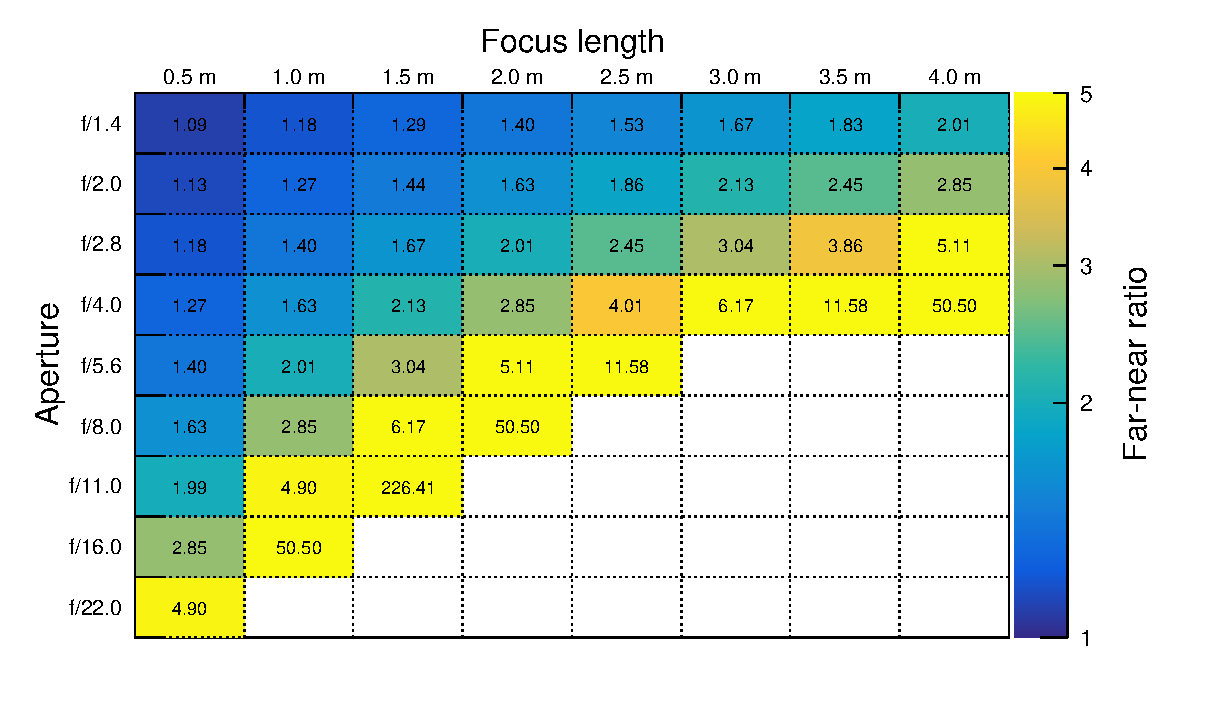
\includegraphics[center,width=0.78\textwidth]{img/far-near-ratio_focl16.eps}
\end{frame}

\begin{frame}[plain]{}
  \vspace{1ex}
  \centering
  Far-Near ratio | {\bf Focal length = 20 mm} |  Sony $\alpha$\hspace{0.1em}6000 (aps-c) | CoC = 0.036 mm
  
  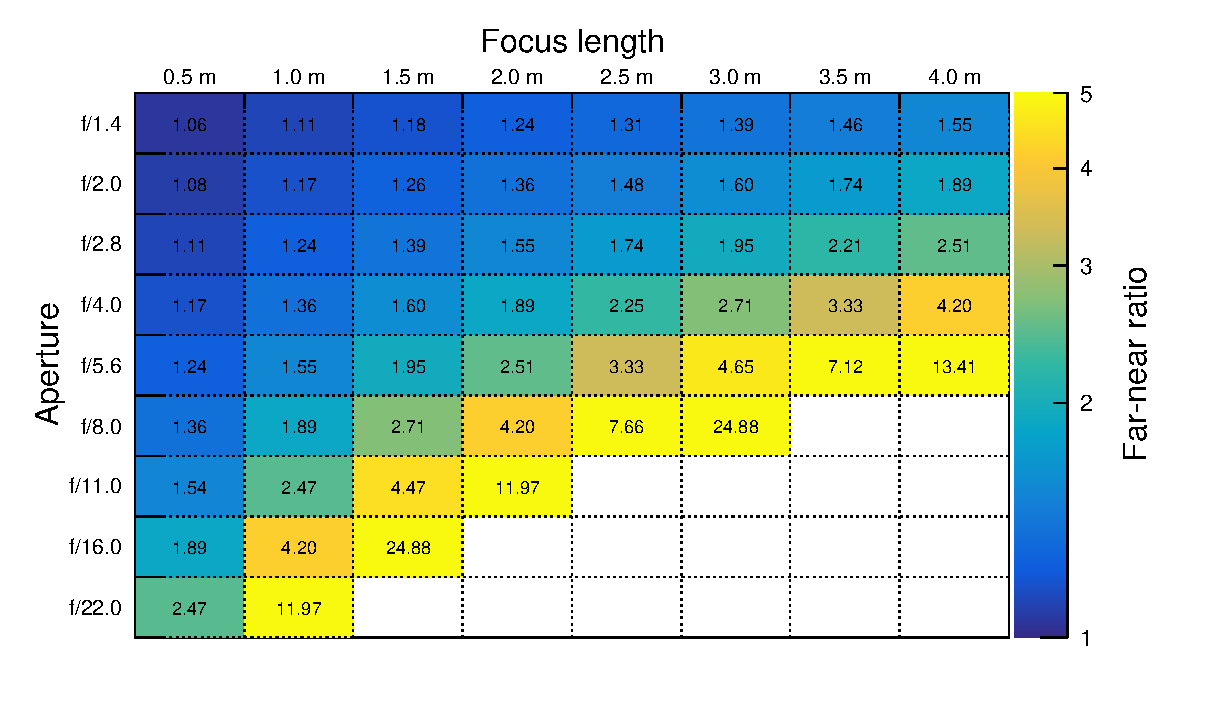
\includegraphics[center,width=0.78\textwidth]{img/far-near-ratio_focl20.eps}
\end{frame}

\begin{frame}[plain]{}
  \vspace{1ex}
  \centering
  Far-Near ratio | {\bf Focal length = 30 mm} |  Sony $\alpha$\hspace{0.1em}6000 (aps-c) | CoC = 0.036 mm
  
  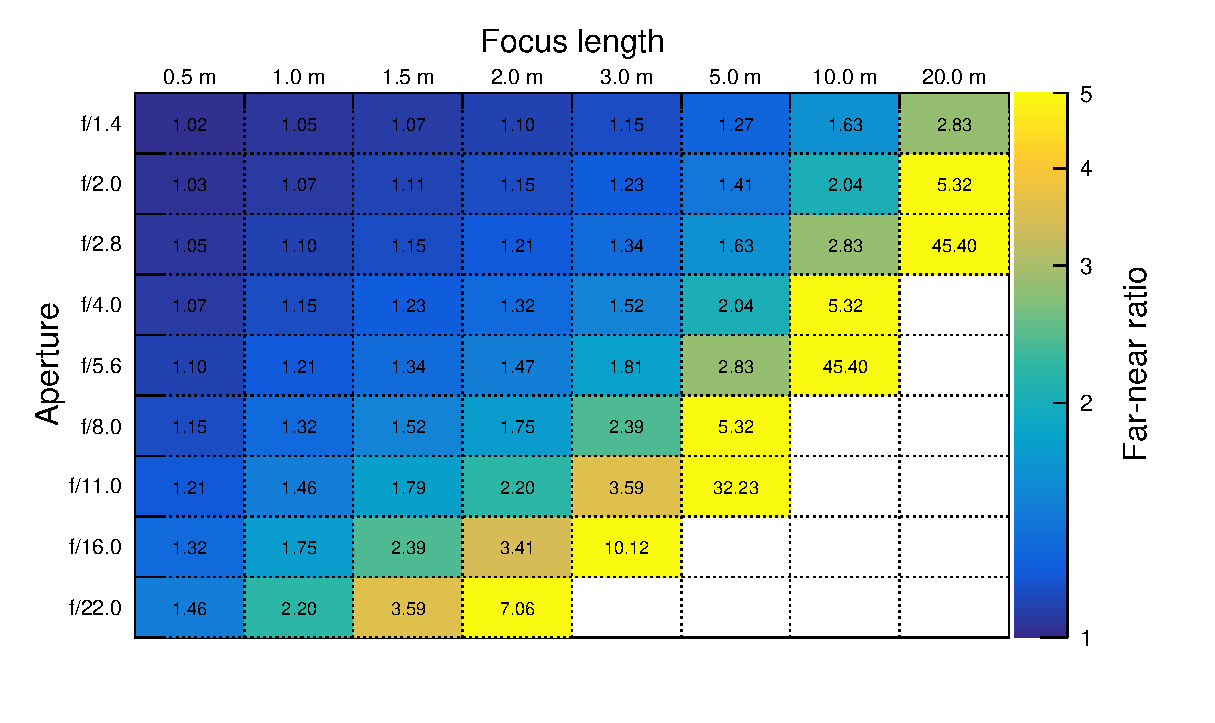
\includegraphics[center,width=0.78\textwidth]{img/far-near-ratio_focl30.eps}
\end{frame}

\begin{frame}[plain]{}
  \vspace{1ex}
  \centering
  Far-Near ratio | {\bf Focal length = 40 mm} |  Sony $\alpha$\hspace{0.1em}6000 (aps-c) | CoC = 0.036 mm
  
  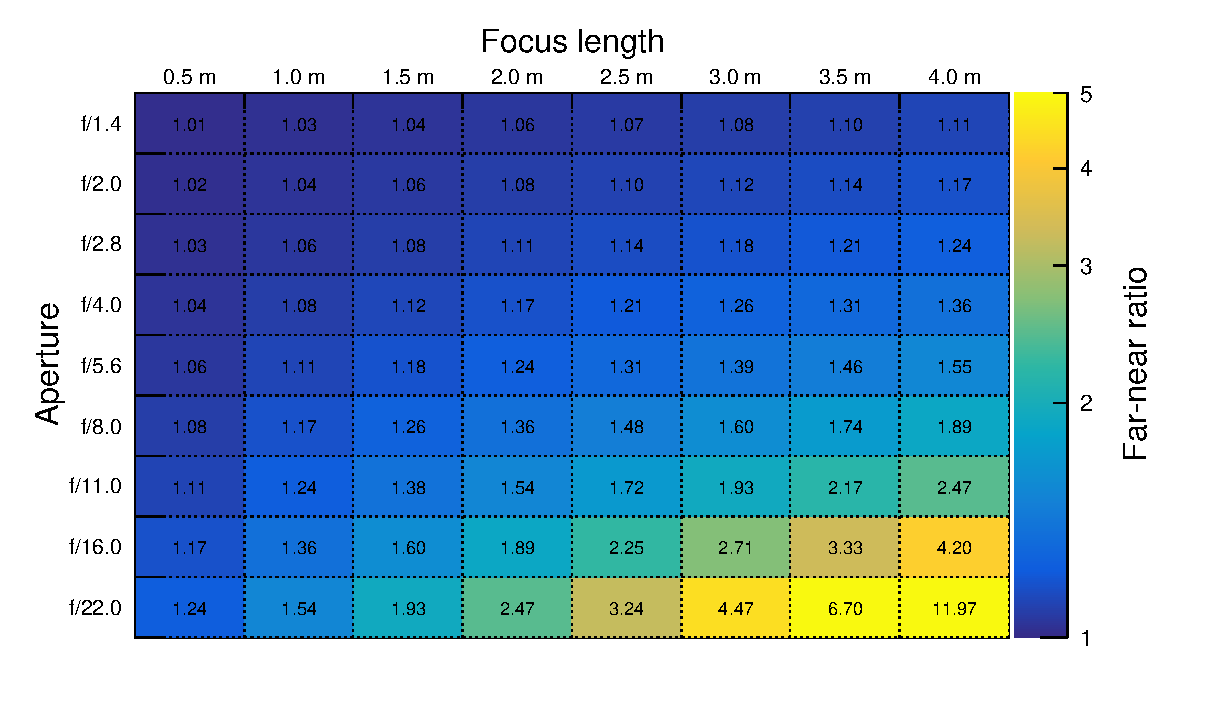
\includegraphics[center,width=0.78\textwidth]{img/far-near-ratio_focl40.eps}
\end{frame}

\begin{frame}[plain]{}
  \vspace{1ex}
  \centering
  Far-Near ratio | {\bf Focal length = 50 mm} |  Sony $\alpha$\hspace{0.1em}6000 (aps-c) | CoC = 0.036 mm
  
  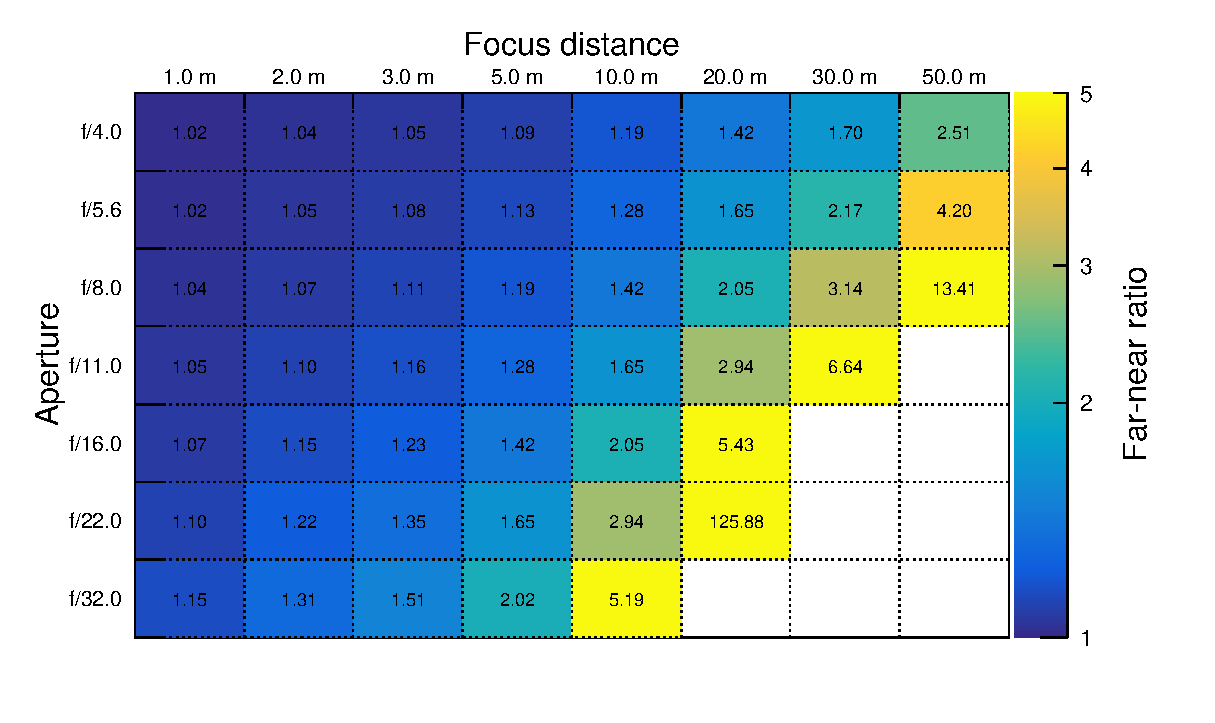
\includegraphics[center,width=0.78\textwidth]{img/far-near-ratio_focl50.eps}
\end{frame}

\begin{frame}[plain]{}
  \vspace{1ex}
  \centering
  Far-Near ratio | {\bf Focal length = 100 mm} |  Sony $\alpha$\hspace{0.1em}6000 (aps-c) | CoC = 0.036 mm
  
  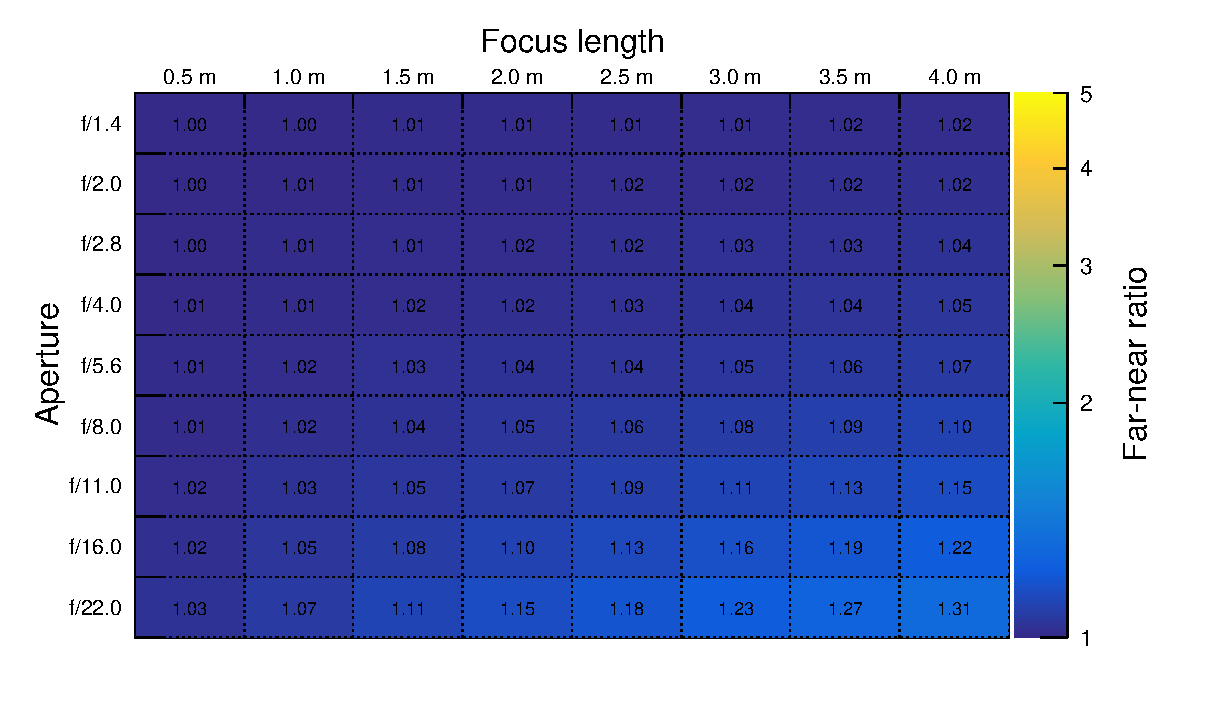
\includegraphics[center,width=0.78\textwidth]{img/far-near-ratio_focl100.eps}
\end{frame}

\begin{frame}[plain]{}
  \vspace{1ex}
  \centering
  Far-Near ratio | {\bf Focal length = 210 mm} |  Sony $\alpha$\hspace{0.1em}6000 (aps-c) | CoC = 0.036 mm
  
  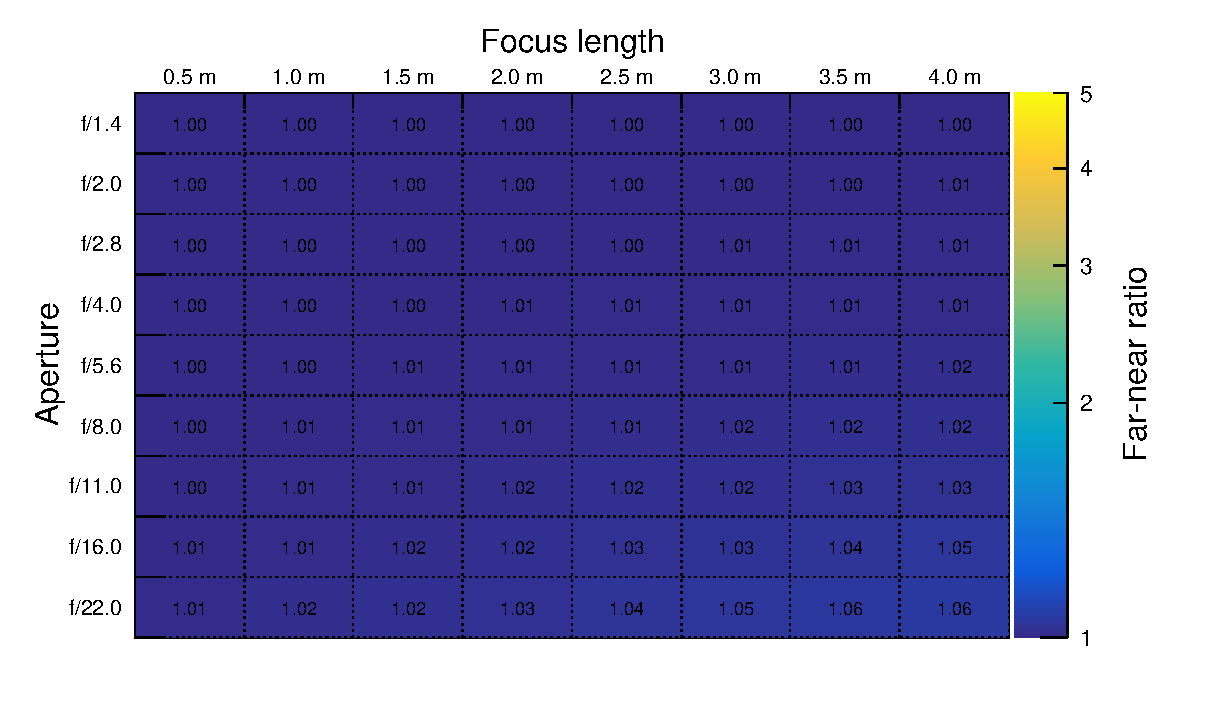
\includegraphics[center,width=0.78\textwidth]{img/far-near-ratio_focl210.eps}
\end{frame}

\end{document}
